\documentclass[11pt,letterpaper]{article}

\usepackage{graphicx}
\usepackage[margin=1in]{geometry}
\usepackage{amsmath}
\usepackage[T1]{fontenc}
\usepackage[utf8]{inputenc}
\usepackage{authblk}
\usepackage{fancyhdr}
\usepackage{lastpage}
\usepackage[parfill]{parskip}
\usepackage{subcaption}
\usepackage{color}

\pagestyle{fancyplain}

% Headers
\lhead{}
\chead{}
\rhead{}

% Footers
\lfoot{}
\cfoot{}
\rfoot{\footnotesize Page \thepage\ of \pageref{LastPage}}

\renewcommand{\headrulewidth}{0.0pt} % No header rule
\renewcommand{\footrulewidth}{0.4pt} % Thin footer rule

\title{Federated Consistency Simulation: \\
 The Effect of Latency and Timing Parameters on Consistency}
\date{August 15, 2016}
\author[ ]{Benjamin Bengfort}
\author[ ]{Pete Keleher}
\affil[ ]{Department of Computer Science}
\affil[ ]{University of Maryland}
\affil[ ]{\textit{\{bengfort,keleher\}@cs.umd.edu}}

\begin{document}

\maketitle

These results show the effect of the network environment in terms of message latency and variability on consistency models. Distributed storage systems must be sensitive to how fast messages can be sent to other replicas on the network and expose that sensitivity through \textit{timing parameters}. Our implementation has three primary timing parameters: \textit{anti-entropy delay} (\texttt{AED}) for Eventually consistent nodes; and \textit{heartbeat interval} (\texttt{HBI}) and \textit{election timeout} (\texttt{ETO}) for Raft nodes (Federated uses all three parameters). These parameters are computed with respect to the network's average message latency ($\lambda_{\mu}$) and standard deviation ($\lambda_{\sigma}$) via a tick parameter ($T$). We currently implement two primary mechanisms for computing $T$), ``bailis'' and ``howard'' referring to the authors of papers who discussed these models.

\begin{equation}T_{bailis} = 10\lambda_{\mu}\end{equation}
\begin{equation}T_{howard} = 2(\lambda_{\mu} + 2\lambda{\sigma})\end{equation}

The timing parameters are then computed from $T$ in a standard fashion. Both \texttt{AED} $=\frac{T}{4}$ and \texttt{HBI} $=\frac{T}{2}$ are fractions of the T metric, while the \texttt{ETO} $=U(T, 2T)$ is a uniform random selection in a range specified by $T$. Note that the Raft parameters follow from the discussion of $T$, whereas the anti-entropy parameter was arbitrarily selected. These parameters play a significant role in the performance and correctness of the replication environment; while the ``bailis'' model is significantly more conservative, the ``howard'' model suffers from critical failures; and in fact several of the ``howard'' simulations for both Federated and Raft failed due to message thrashing of the followers (out of order \texttt{AppendEntries} messages).

The independent variable in these simulations is the $\lambda_{\mu}$ and $\lambda_{\sigma}$ of the \textit{wide area network} (specified primarily by $\lambda_{\mu}$). The fixed variables are as follows: local area links remain fixed with a normal distribution of $\lambda_{\mu} = 15ms$, $\lambda_{\sigma} = 2ms$. The simulation topology is set up with 20 nodes, 4 each in 5 locations; all fully connected (see Figure \ref{fig:topology} for topological details). All 20 nodes generate accesses on 28 objects (48,038 total accesses) with a conflict probability, $P_c = 0.5$, meaning that each object is accessed on average by 7 devices. The interval between accesses for each node is normally distributed, $A_{\mu}=1800ms$, $A_{\sigma}=240ms$. Accesses to objects are sequenced, with probability of switching objects, $P_o=0.1$ and the probability of a read, $P_r=0.58$. All simulations use an identical trace file generated with these parameters called ``moderate conflict workload''.

The wide area network latencies are solely used to compute $T$ and therefore the timing parameters are also only dependent on the wide area. For each tick parameter model (``bailis'' and ``howard''), three latency/variation ranges for the wide area network were constructed with 12 simulations in each (for a total of 216 simulations). The wide area ranges are as follows:

\begin{itemize}
    \item $\lambda_{\mu} = [60,973]ms$, $\lambda_{\sigma}=16ms$
    \item $\lambda_{\mu} = [1080,1993]ms$, $\lambda_{\sigma}=32ms$
    \item $\lambda_{\mu} = [2120,3033]ms$, $\lambda_{\sigma}=48ms$
\end{itemize}

The ranges for $\lambda_{\mu}$ were constructed with equal width and a step $=83$; the width of the wide area mean latency range is 36 intervals between 60 and 3033 milliseconds.

These 216 simulations were run on the new bluejacket.cs.umd.edu virtual machine (1 day 4 hours 12 minutes 48 seconds compute time) by 8 tasks for a real time computation of 4 hours 52 minutes 8 seconds.

\textcolor{red}{31 simulations, all with ``howard'' timing parameters (both Raft and Federated), failed due to a consistency violation exception in the log.} The violation is caused when out of order \texttt{AppendEntries} messages cause a follower node to reject the message because the follower believes they are behind (e.g. the \texttt{AppendEntries.lastLogIndex} is ahead of the log index of the follower). The follower begins the log reconciliation process with the leader, only to receive the late \texttt{AppendEntries}, and updates the log with the correct information. The leader, seeing a failed \texttt{AppendEntries} decrements the log index to reconcile the follower, and sends an update. A consistency conflict has now occurred from the point of view of the follower, therefore they delete (the correct) log entry and send a reconciliation request, which is now out of order yet again. This causes the leader and the follower to thrash the follower's log until it is completely empty.

This effect, as well as election thrashing are the primary reason that the timing parameter for Raft is set so high (along with the resulting poor performance). Raft implementations may choose to deal with this issue either by replaying the entire log once it has been pushed to zero (and caching the log on each election) or by keeping a monotonically increasing message number in addition to the term/last index information. We have not made a choice how to deal with this in our simulation.

Figures for the completed 185 simulations results follow.

\begin{figure}[!h]
    \centering
        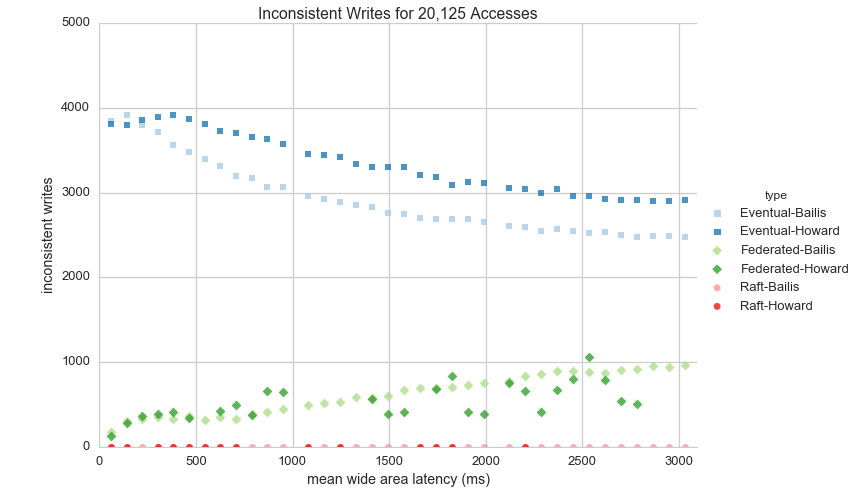
\includegraphics[width=\textwidth]{figures/inconsistent_writes.png}
        \caption{\textsf{An \textbf{inconsistent write} is a write that has been accepted by a node that would lead to a fork. Raft does not allow inconsistent writes, however Eventual nodes will allow them into their logs. For eventual, it appears that the longer the anti-entropy delay, the fewer inconsistent writes exist (the anti-entropy delay increases as $T$ increases, which in turn increases as $\lambda_{\mu}$ and $\lambda_{\sigma}$ increase). \\
\\
        I'm at a bit of a loss to explain this, as I would hypothesize that inconsistencies would increase with more message delay. Note that inconsistent writes in Eventual is equivalent to forks shown in Figure \ref{fig:forked_writes}, which generally speaking are the direct results of stale reads. Stale reads do increase for Eventual with respect to $\lambda_{\mu}$ as shown in Figure \ref{fig:stale_reads}. I will look more into this to see if I can figure out what is going on.\\
\\
        Federated does show an increasing number of inconsistencies as the wide area latency increases, though the ``howard'' model is fairly unstable. Because Raft will not let any inconsistent writes into their logs, these inconsistencies must come entirely from Eventual nodes.}}
        \label{fig:inconsistent_writes}
\end{figure}

\begin{figure}[!h]
    \centering
        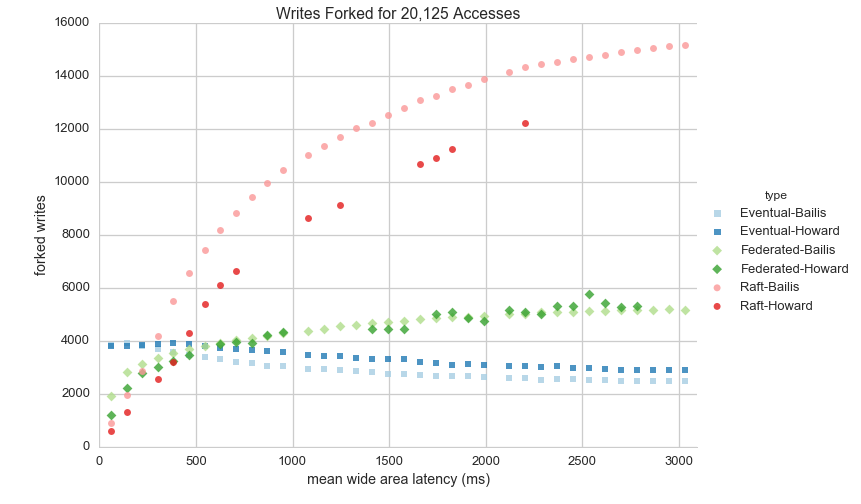
\includegraphics[width=\textwidth]{figures/forked_writes.png}
        \caption{\textsf{A \textbf{fork} in the version history for a single object is caused when a replica writes to a stale version that is cached locally. Forks occur primarily because of conflict and in Eventual, the potential for forks can quickly be stomped on due to the latest version wins heuristic of the simulation. However, in Raft land, with a leader aggregating writes for \texttt{AppendEntries}, the possibility of forks/stale reads increases as that delay increases - a delay that is related to the mean latency in a significant way.}}
        \label{fig:forked_writes}
\end{figure}


\begin{figure}[!h]
    \centering
        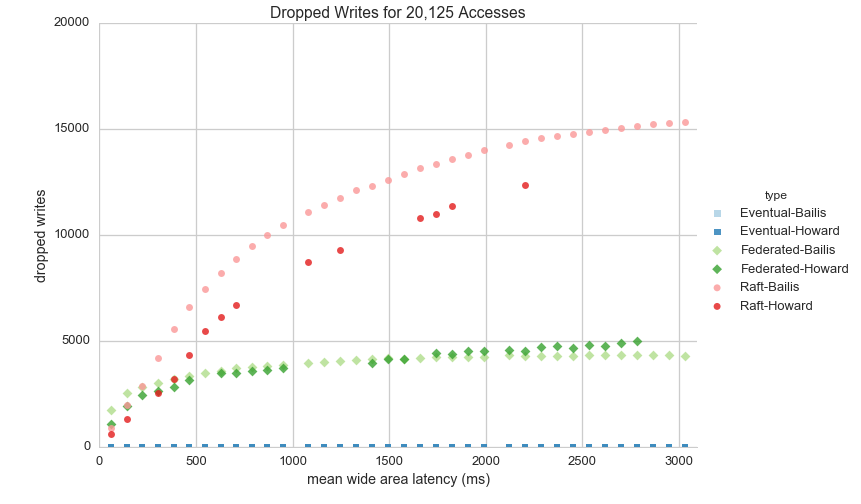
\includegraphics[width=\textwidth]{figures/dropped_writes.png}
        \caption{\textsf{A \textbf{dropped write} is a rejection of a write due to it not meeting some consistency criteria. Raft rejects all forks, therefore it is equivalent to the number of forks. Eventual on the other hand does not reject any writes, though it does capture inconsistency. Federated sits between Raft and Eventual by minimizing inconsistencies and dropped writes by minimizing the number of forks via enforced ordering and fewer stale reads.}}
        \label{fig:dropped_writes}
\end{figure}

\begin{figure}[!h]
    \centering
        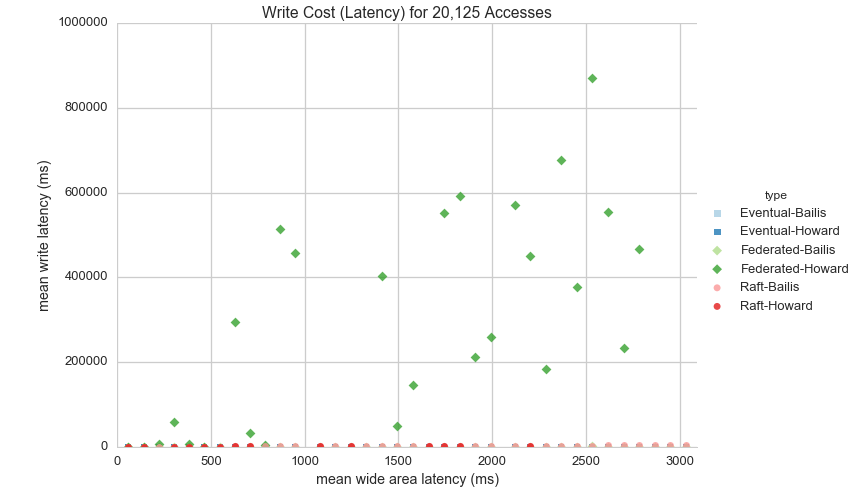
\includegraphics[width=\textwidth]{figures/write_latency.png}
        \caption{\textsf{Here we can really only see the effect of network instability on the more optimistic ``howard'' parameter. The more variable the network, the more likely that message thrashing occurs, and therefore the inability for Raft to recover. It appears that most of the Raft-Howard high latency/variability simulations simply failed (e.g. not a whole lot of solid red dots). It may be interesting to note that Federated actually appears to have recovered somewhat from message thrashing; potentially because those nodes are also participating in anti-entropy therefore have a mechanism to reconcile logs stopping the out of order \texttt{AppendEntries}? Alternatively, it could simply be that there are fewer Raft nodes in Federated, and therefore a smaller likelihood of the type of thrashing that leads to fatal inconsistency errors.}}
        \label{fig:write_latency}
\end{figure}


\begin{figure}[!h]
    \centering
        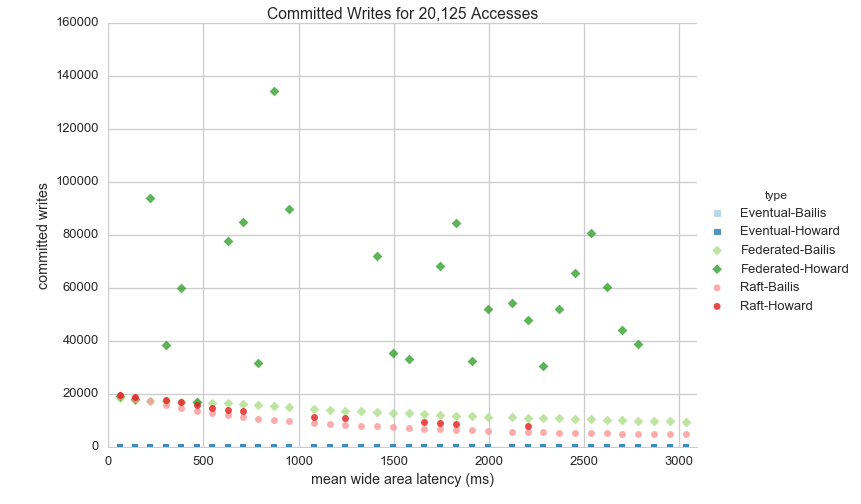
\includegraphics[width=\textwidth]{figures/committed_writes.png}
        \caption{\textsf{Once again, this graph is showing the message thrashing due to the Howard parameter. The reason that there are triple the number of committed writes with Howard is because part of the log is being replayed after an out-of-order \texttt{AppendEntries}, causing the write to be ``committed'' again.}}
        \label{fig:committed_writes}
\end{figure}

\begin{figure}[!h]
    \centering
        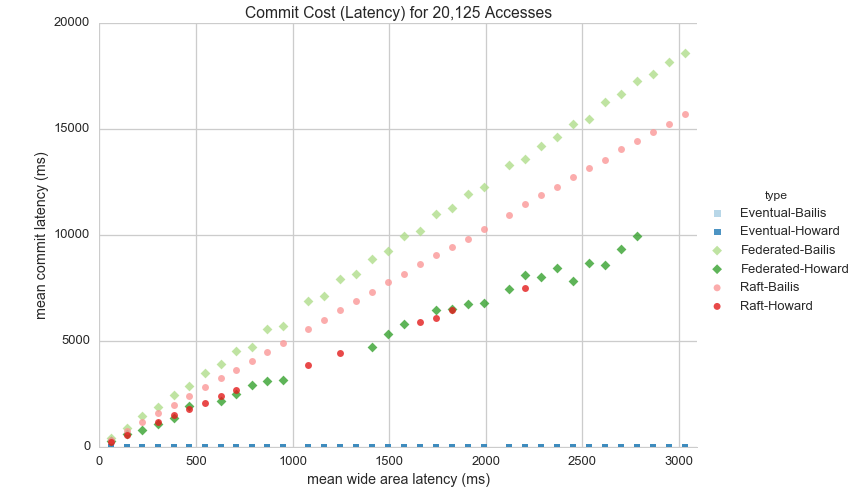
\includegraphics[width=\textwidth]{figures/commit_latency.png}
        \caption{\textsf{This graph is a function of how I'm recording results; though a ``commit'' might occur multiple times, the commit latency is recorded as the time delta from when the access occurred to when it was first seen as committed by the leader; therefore the time delta was always the same, and the mean commit latency remains unchanged though the number of records increases. Commit latency is the cost of two \texttt{AppendEntries} messages, so the higher the $T$ parameter, the longer the commit latency.}}
        \label{fig:commit_latency}
\end{figure}

\begin{figure}[!h]
    \centering
        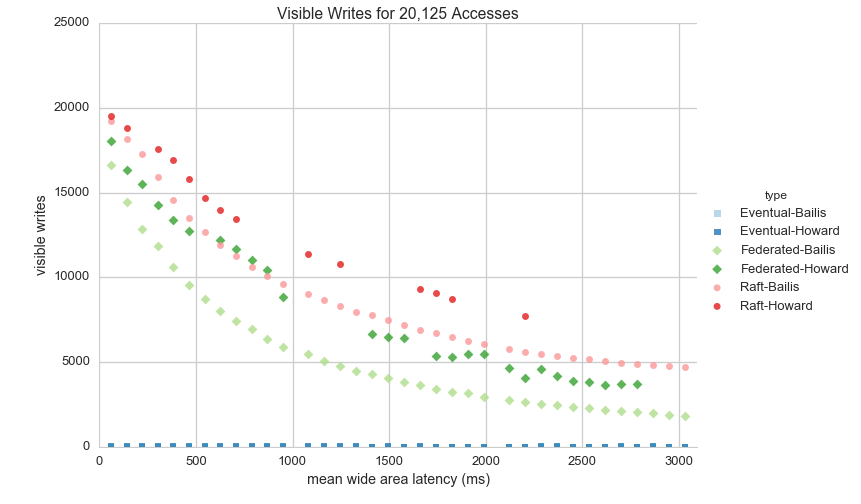
\includegraphics[width=\textwidth]{figures/visible_writes.png}
        \caption{\textsf{Complete visibility bug still not addressed at the time of this simulation for Eventual nodes. Every write should be fully visible for Raft, except for dropped writes. Therefore this curve is showing that the number of dropped writes increases as the mean wide area latency increases, and therefore reduces the total number of visible writes. }}
        \label{fig:visible_writes}
\end{figure}

\begin{figure}[!h]
    \centering
        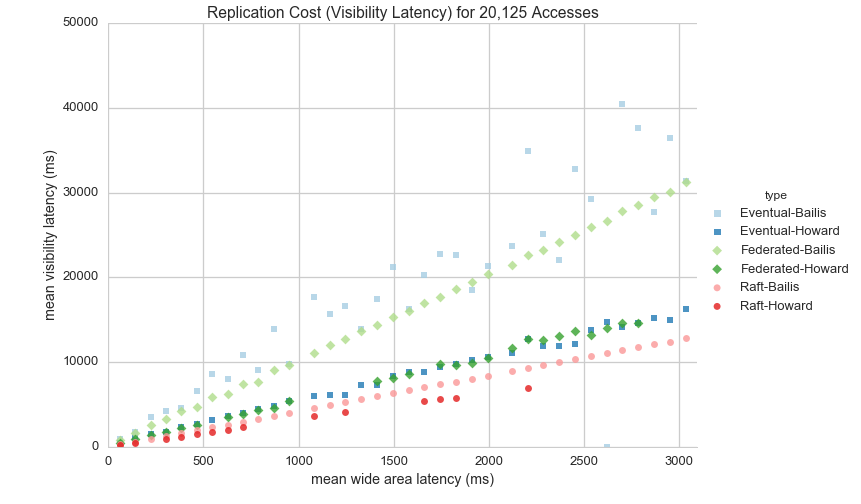
\includegraphics[width=\textwidth]{figures/visibility_latency.png}
        \caption{\textsf{For Raft, visibility is a function of the heartbeat interval because a write becomes fully visible after every node receives an \texttt{AppendEntries} broadcast message.}}
        \label{fig:visibility_latency}
\end{figure}

\begin{figure}[!h]
    \centering
        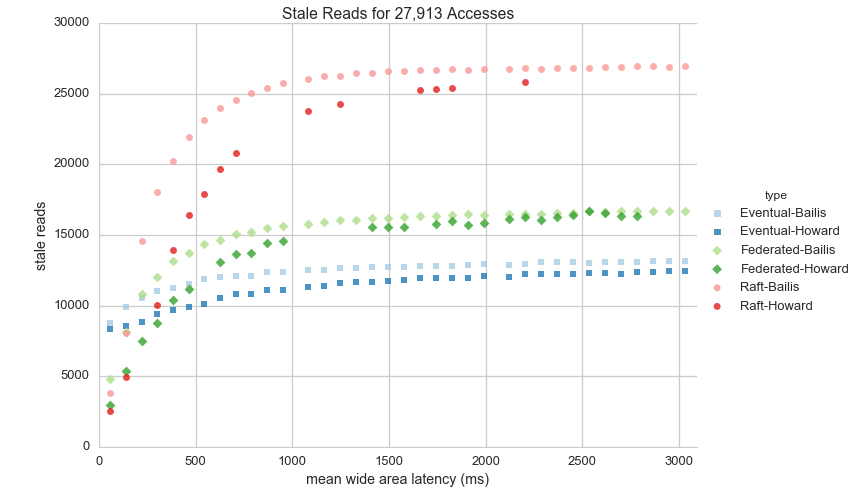
\includegraphics[width=\textwidth]{figures/stale_reads.png}
        \caption{\textsf{A \textbf{stale read} occurs when a read access is triggered and the latest version of the object in the log of the replica is not the latest version globally. Stale reads also contribute to forks since writes model writes-follow-reads.}}
        \label{fig:stale_reads}
\end{figure}

\begin{figure}[!h]
    \centering
        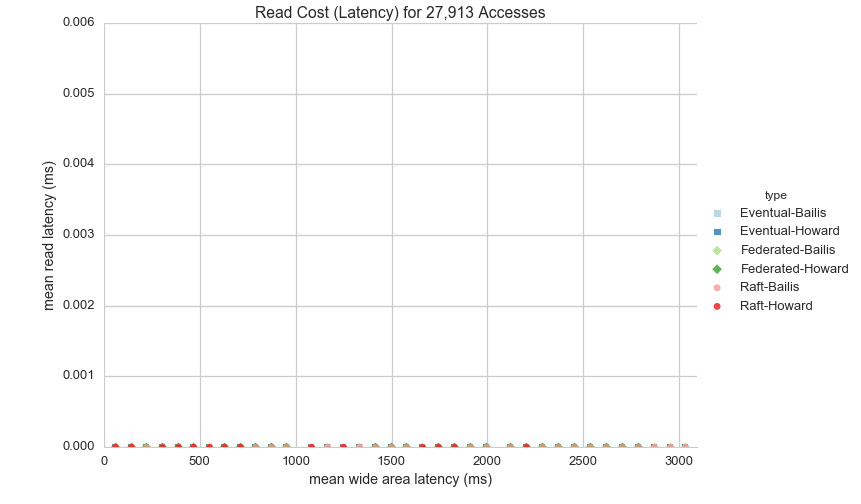
\includegraphics[width=\textwidth]{figures/read_latency.png}
        \caption{\textsf{All nodes read the latest locally cached version, there are no remote reads in the current simulation.}}
        \label{fig:read_latency}
\end{figure}

\begin{figure}[!h]
    \centering
        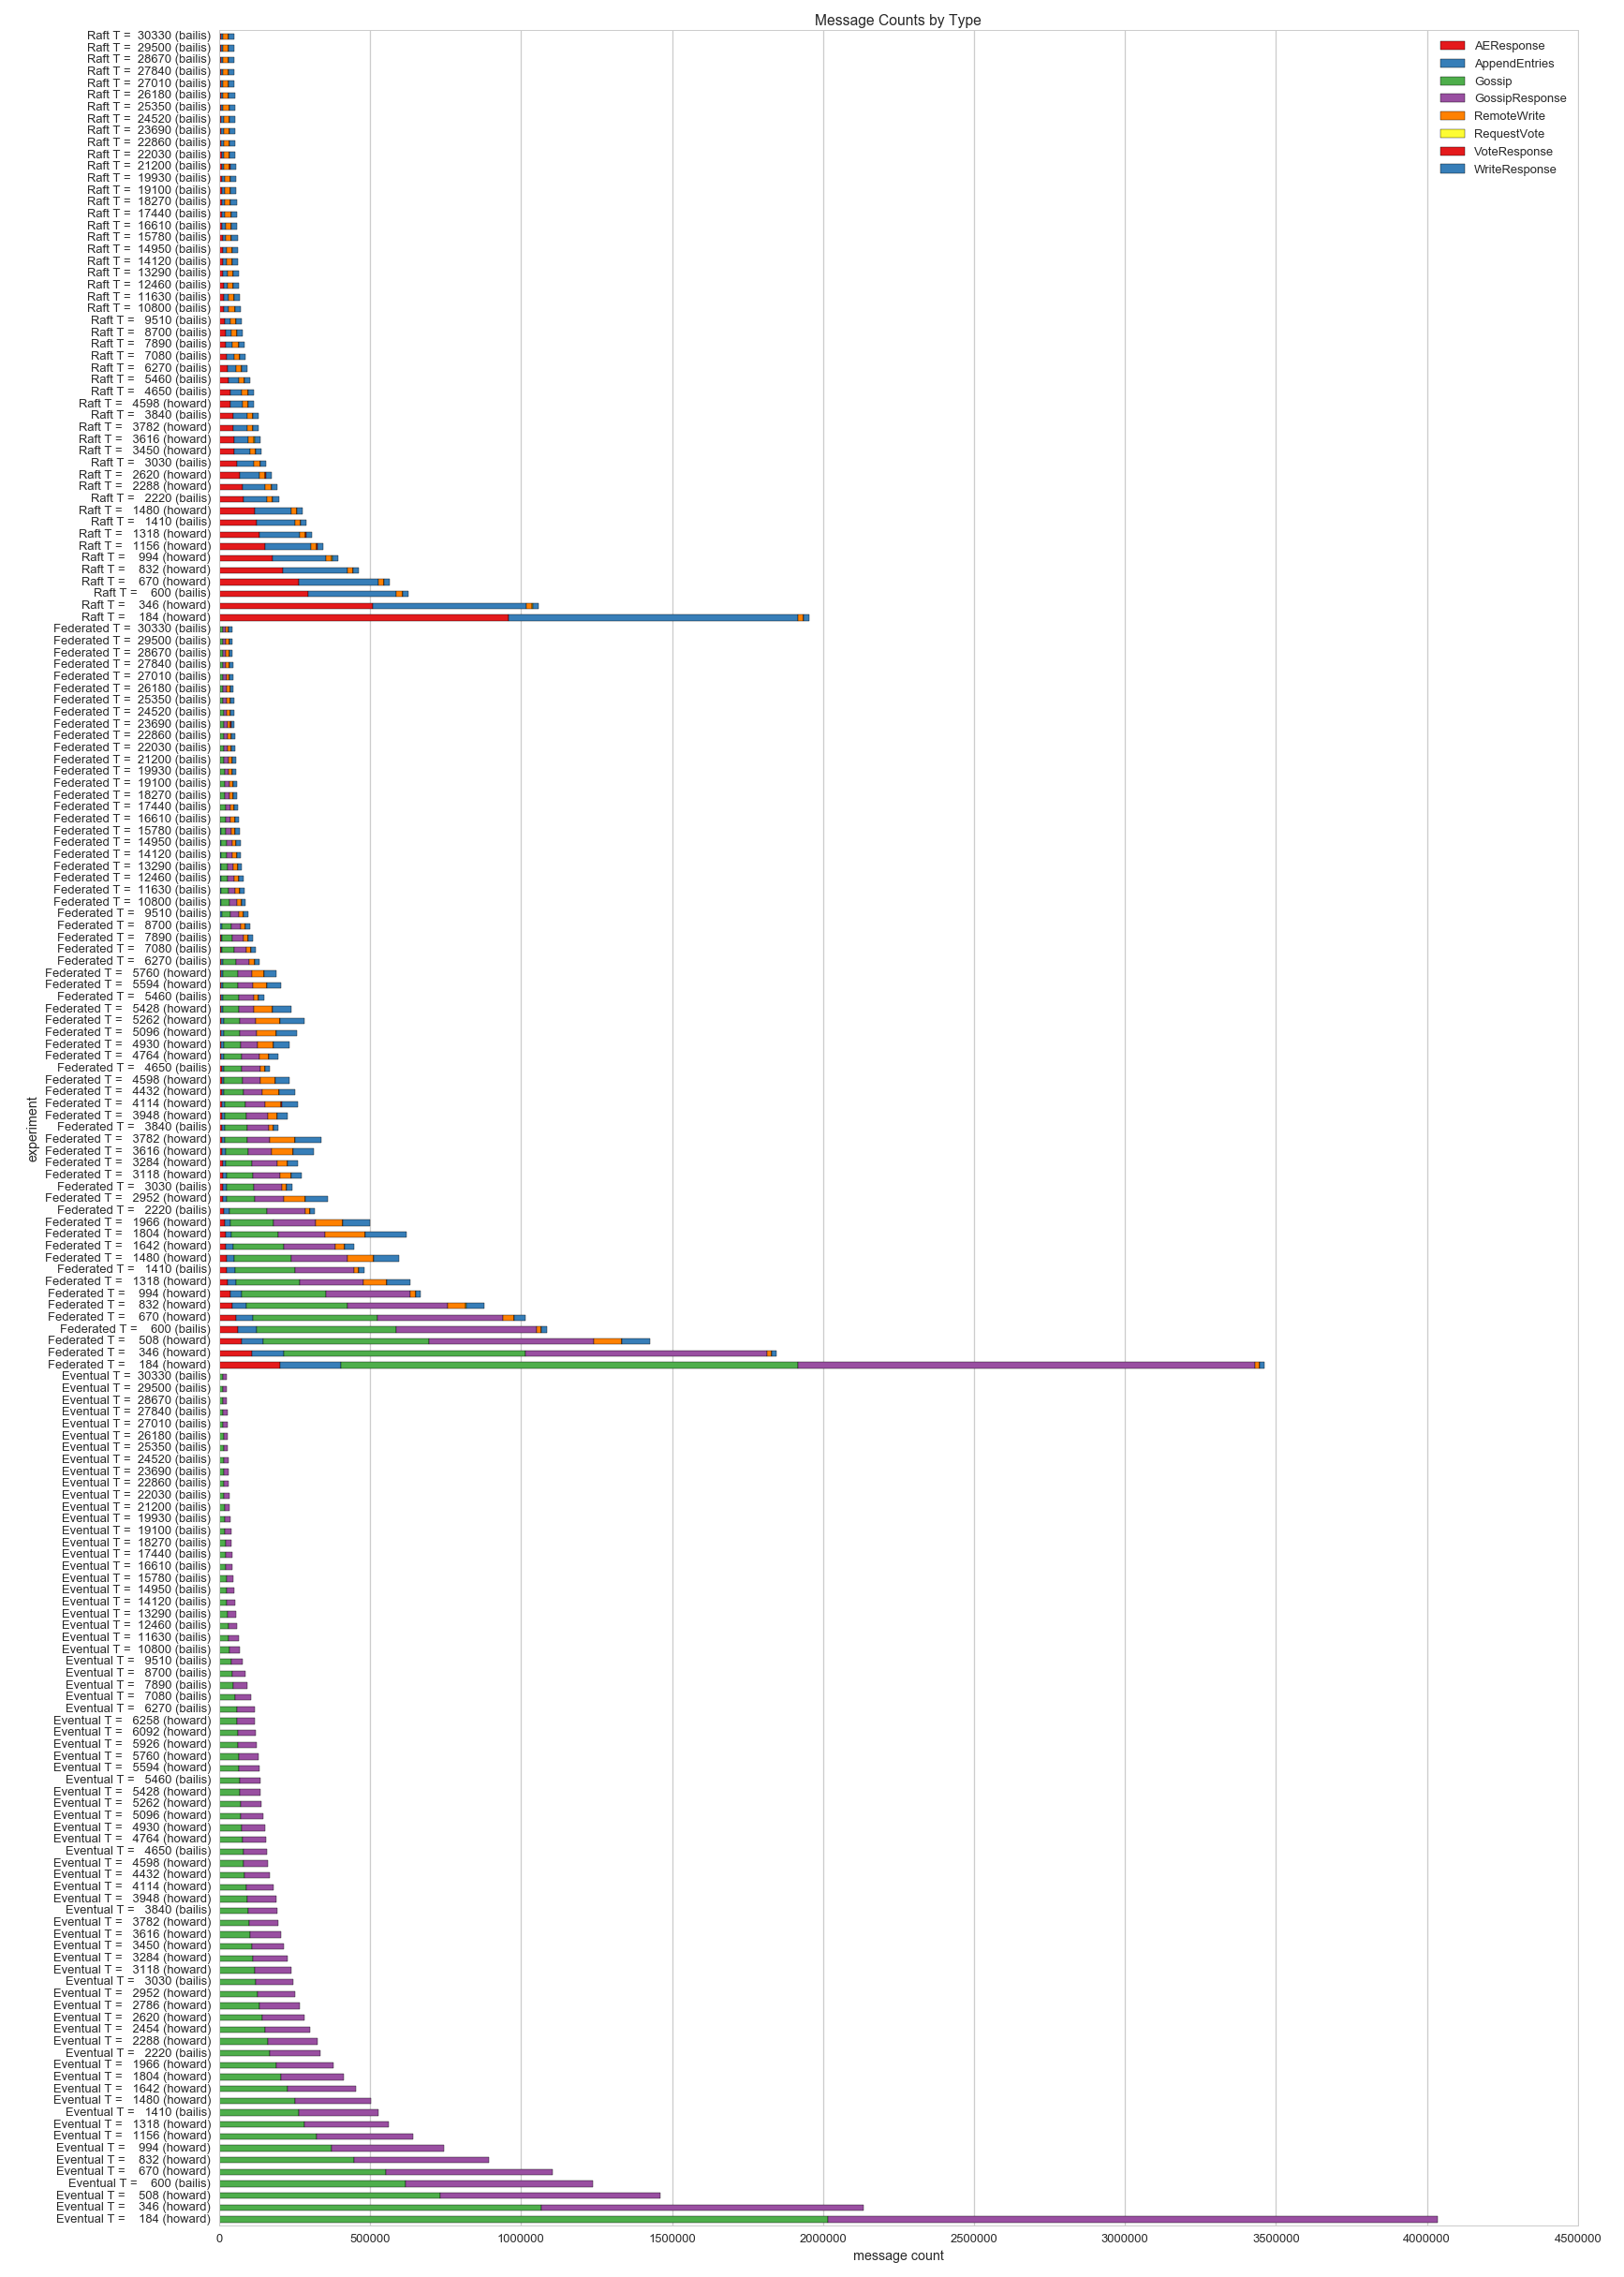
\includegraphics[height=.9\textheight]{figures/message_counts.png}
        \caption{\textsf{See Figure \ref{fig:messages_sent} for more details.}}
        \label{fig:message_counts}
\end{figure}

\begin{figure}[!h]
    \centering
        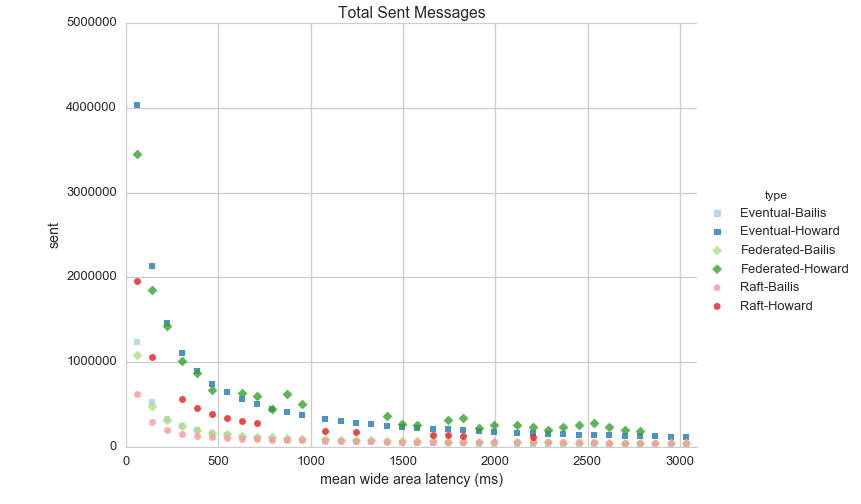
\includegraphics[width=\textwidth]{figures/messages_sent.png}
        \caption{\textsf{As the $T$ parameter increases, the number of messages sent by each replica server exponentially decreases.}}
        \label{fig:messages_sent}
\end{figure}

\begin{figure}[!h]
    \centering
        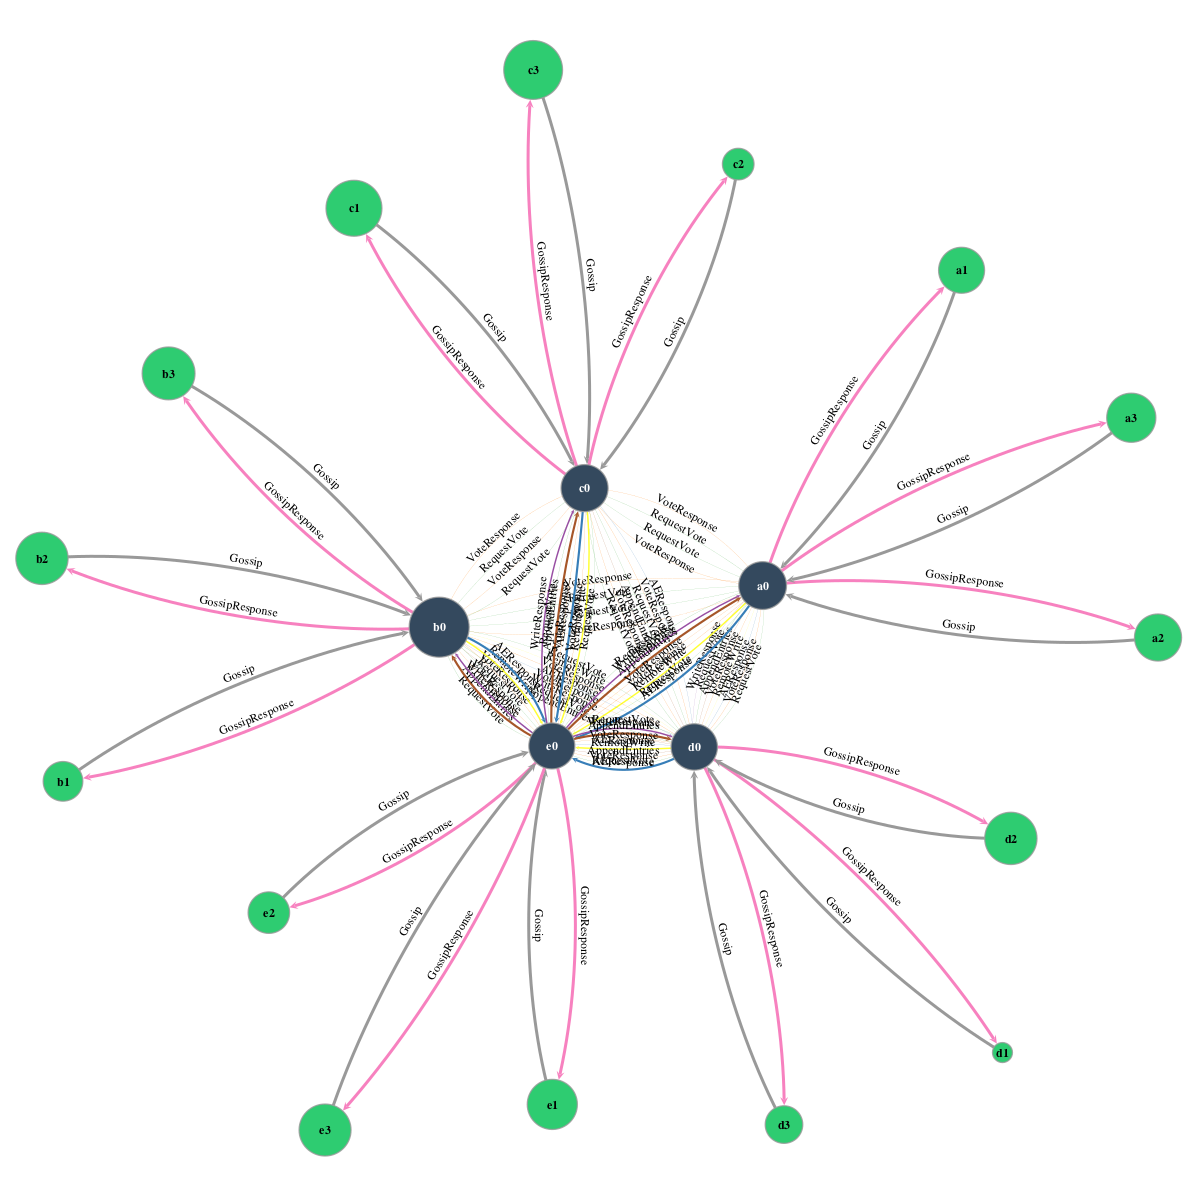
\includegraphics[width=\textwidth]{figures/federated-topology.png}
        \caption{\textsf{The topology of the simulation has 4 nodes connected locally in 5 areas for a total of 20 nodes. All nodes are fully connected and all nodes cause work to occur in the simulation. The federated topology shows the 5 core Raft nodes primarily communicating with each other and their locally connected nodes. Here the size of the node is related to the number of accesses and the size of the edge relates to the number of messages of that type. Node color refers to server implementation. Though nodes are fully connected, wide area anti-entropy is not visible.}}
        \label{fig:topology}
\end{figure}


\end{document}
